%----------------------------------------------------------------------------------------
%	PACKAGES AND THEMES
%----------------------------------------------------------------------------------------

\documentclass{beamer}

\mode<presentation> {
\usetheme{Madrid}

%\setbeamertemplate{footline} % To remove the footer line in all slides uncomment this line
%\setbeamertemplate{footline}[page number] % To replace the footer line in all slides with a simple slide count uncomment this line

\setbeamertemplate{navigation symbols}{} % To remove the navigation symbols from the bottom of all slides uncomment this line
}

\usepackage[ngerman]{babel}
\usepackage[utf8]{inputenc}
\usepackage{graphicx} % Allows including images
\usepackage{booktabs} % Allows the use of \toprule, \midrule and \bottomrule in tables
\usepackage{hyperref}
%----------------------------------------------------------------------------------------
%	TITLE PAGE
%----------------------------------------------------------------------------------------

\title[Assignment2]{Presentation of Assignment 2} % The short title appears at the bottom of every slide, the full title is only on the title page

\author{Ramil Sabirov, Joel Choi, Eric Remigius} % Your name
\institute[] % Your institution as it will appear on the bottom of every slide, may be shorthand to save space
{
RWTH Aachen \\ % Your institution for the title page
\medskip
\textit{Gruppe 3}
}
\date{\today} % Date, can be changed to a custom date

\begin{document}

\begin{frame}
\titlepage % Print the title page as the first slide
\end{frame}

%----------------------------------------------------------------------------------------
%	PRESENTATION SLIDES
%----------------------------------------------------------------------------------------

\begin{frame}
\frametitle{Task 1 - Network}

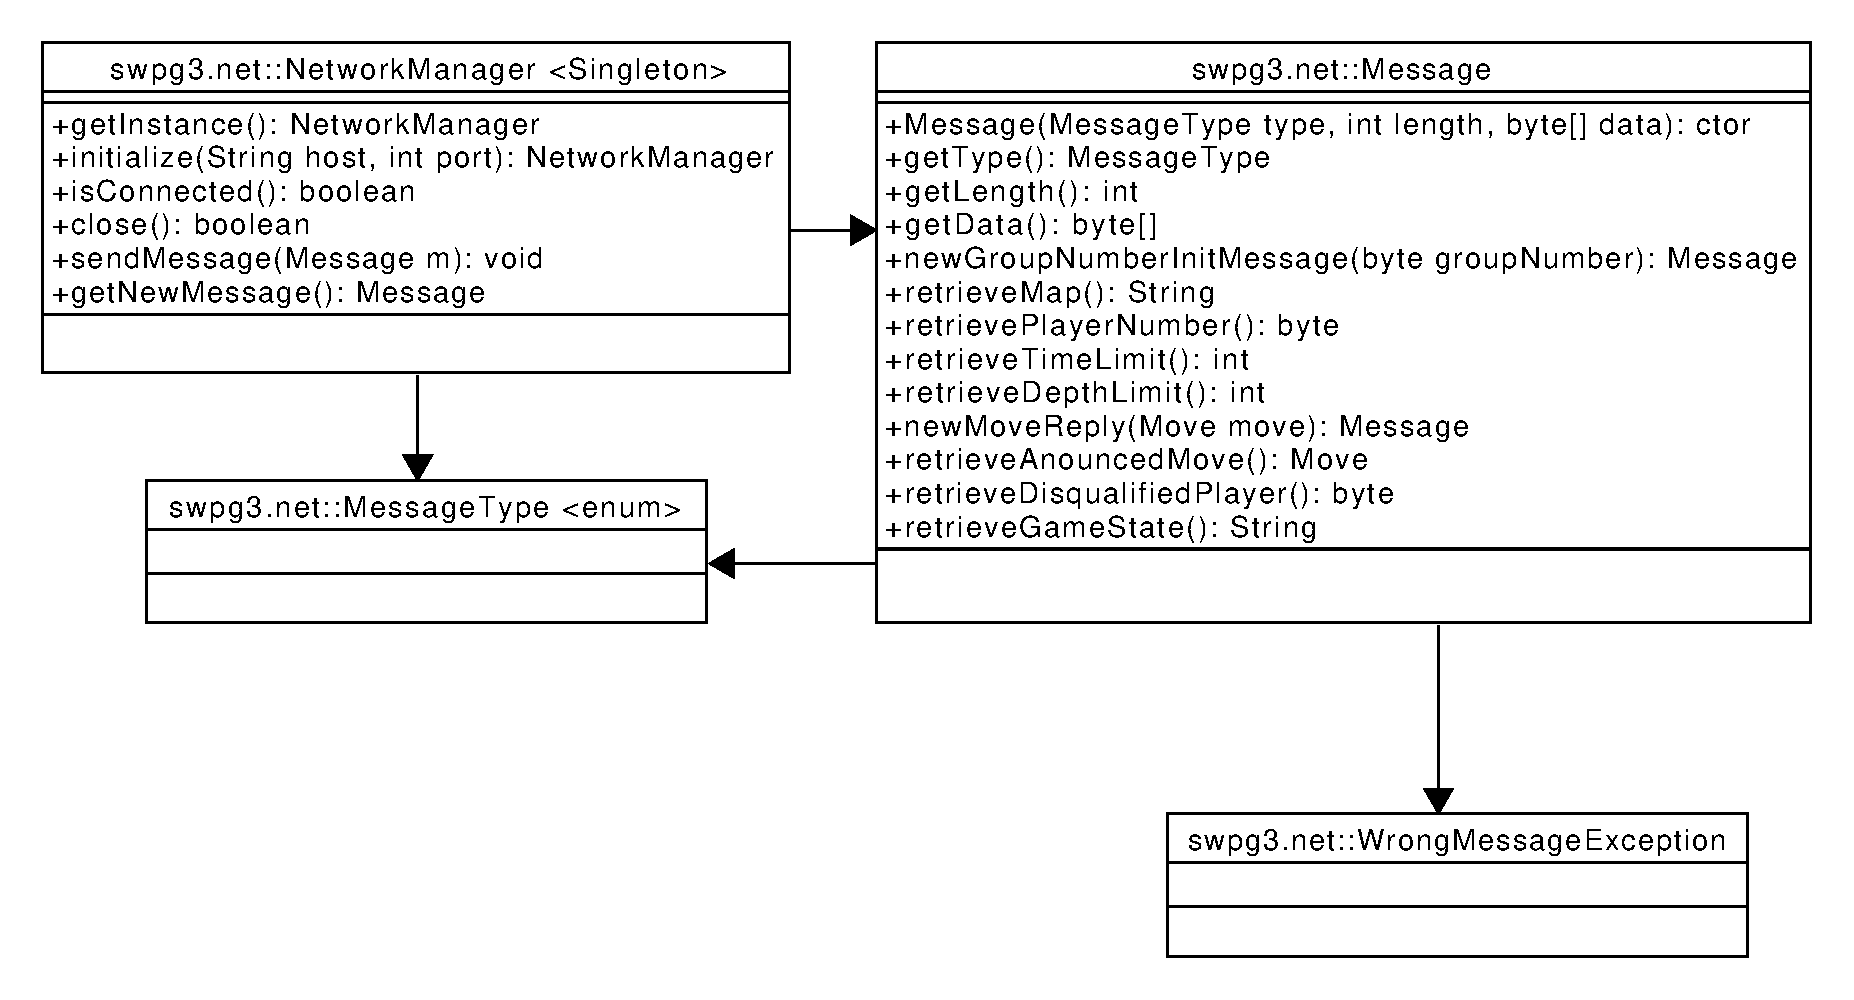
\includegraphics[width=\textwidth]{NetPackageClassdiagramm}

\end{frame}

%------------------------------------------------

\begin{frame}
\frametitle{Task 2 - AI}

\end{frame}

%-------------------------------------------------

\begin{frame}
\frametitle{AI - Bewertungsfunktion}

\textbf{Bewertungskategorien:}
\begin{enumerate}
\item[•] Anzahl eigener Steine
\item[•] "kostenlose" Mobilität
\item[•] Anzahl stabiler Steine
\item[•] Anzahl der Override Steine
\end{enumerate}

\pause
\hfill\break

\textbf{Ablauf der Evaluation:}
\begin{enumerate}
\item[1.] Analyse des Attributes
\item[2.] Auswertung mit Erwartungswertfunktion
\item[3.] Skalierung mit Wichtigkeitsfunktion
\end{enumerate}


\end{frame}

%--------------------------------------------------

\begin{frame}
\frametitle{Bsp. Erwartungswertfunktion - Mobilität}
\centering
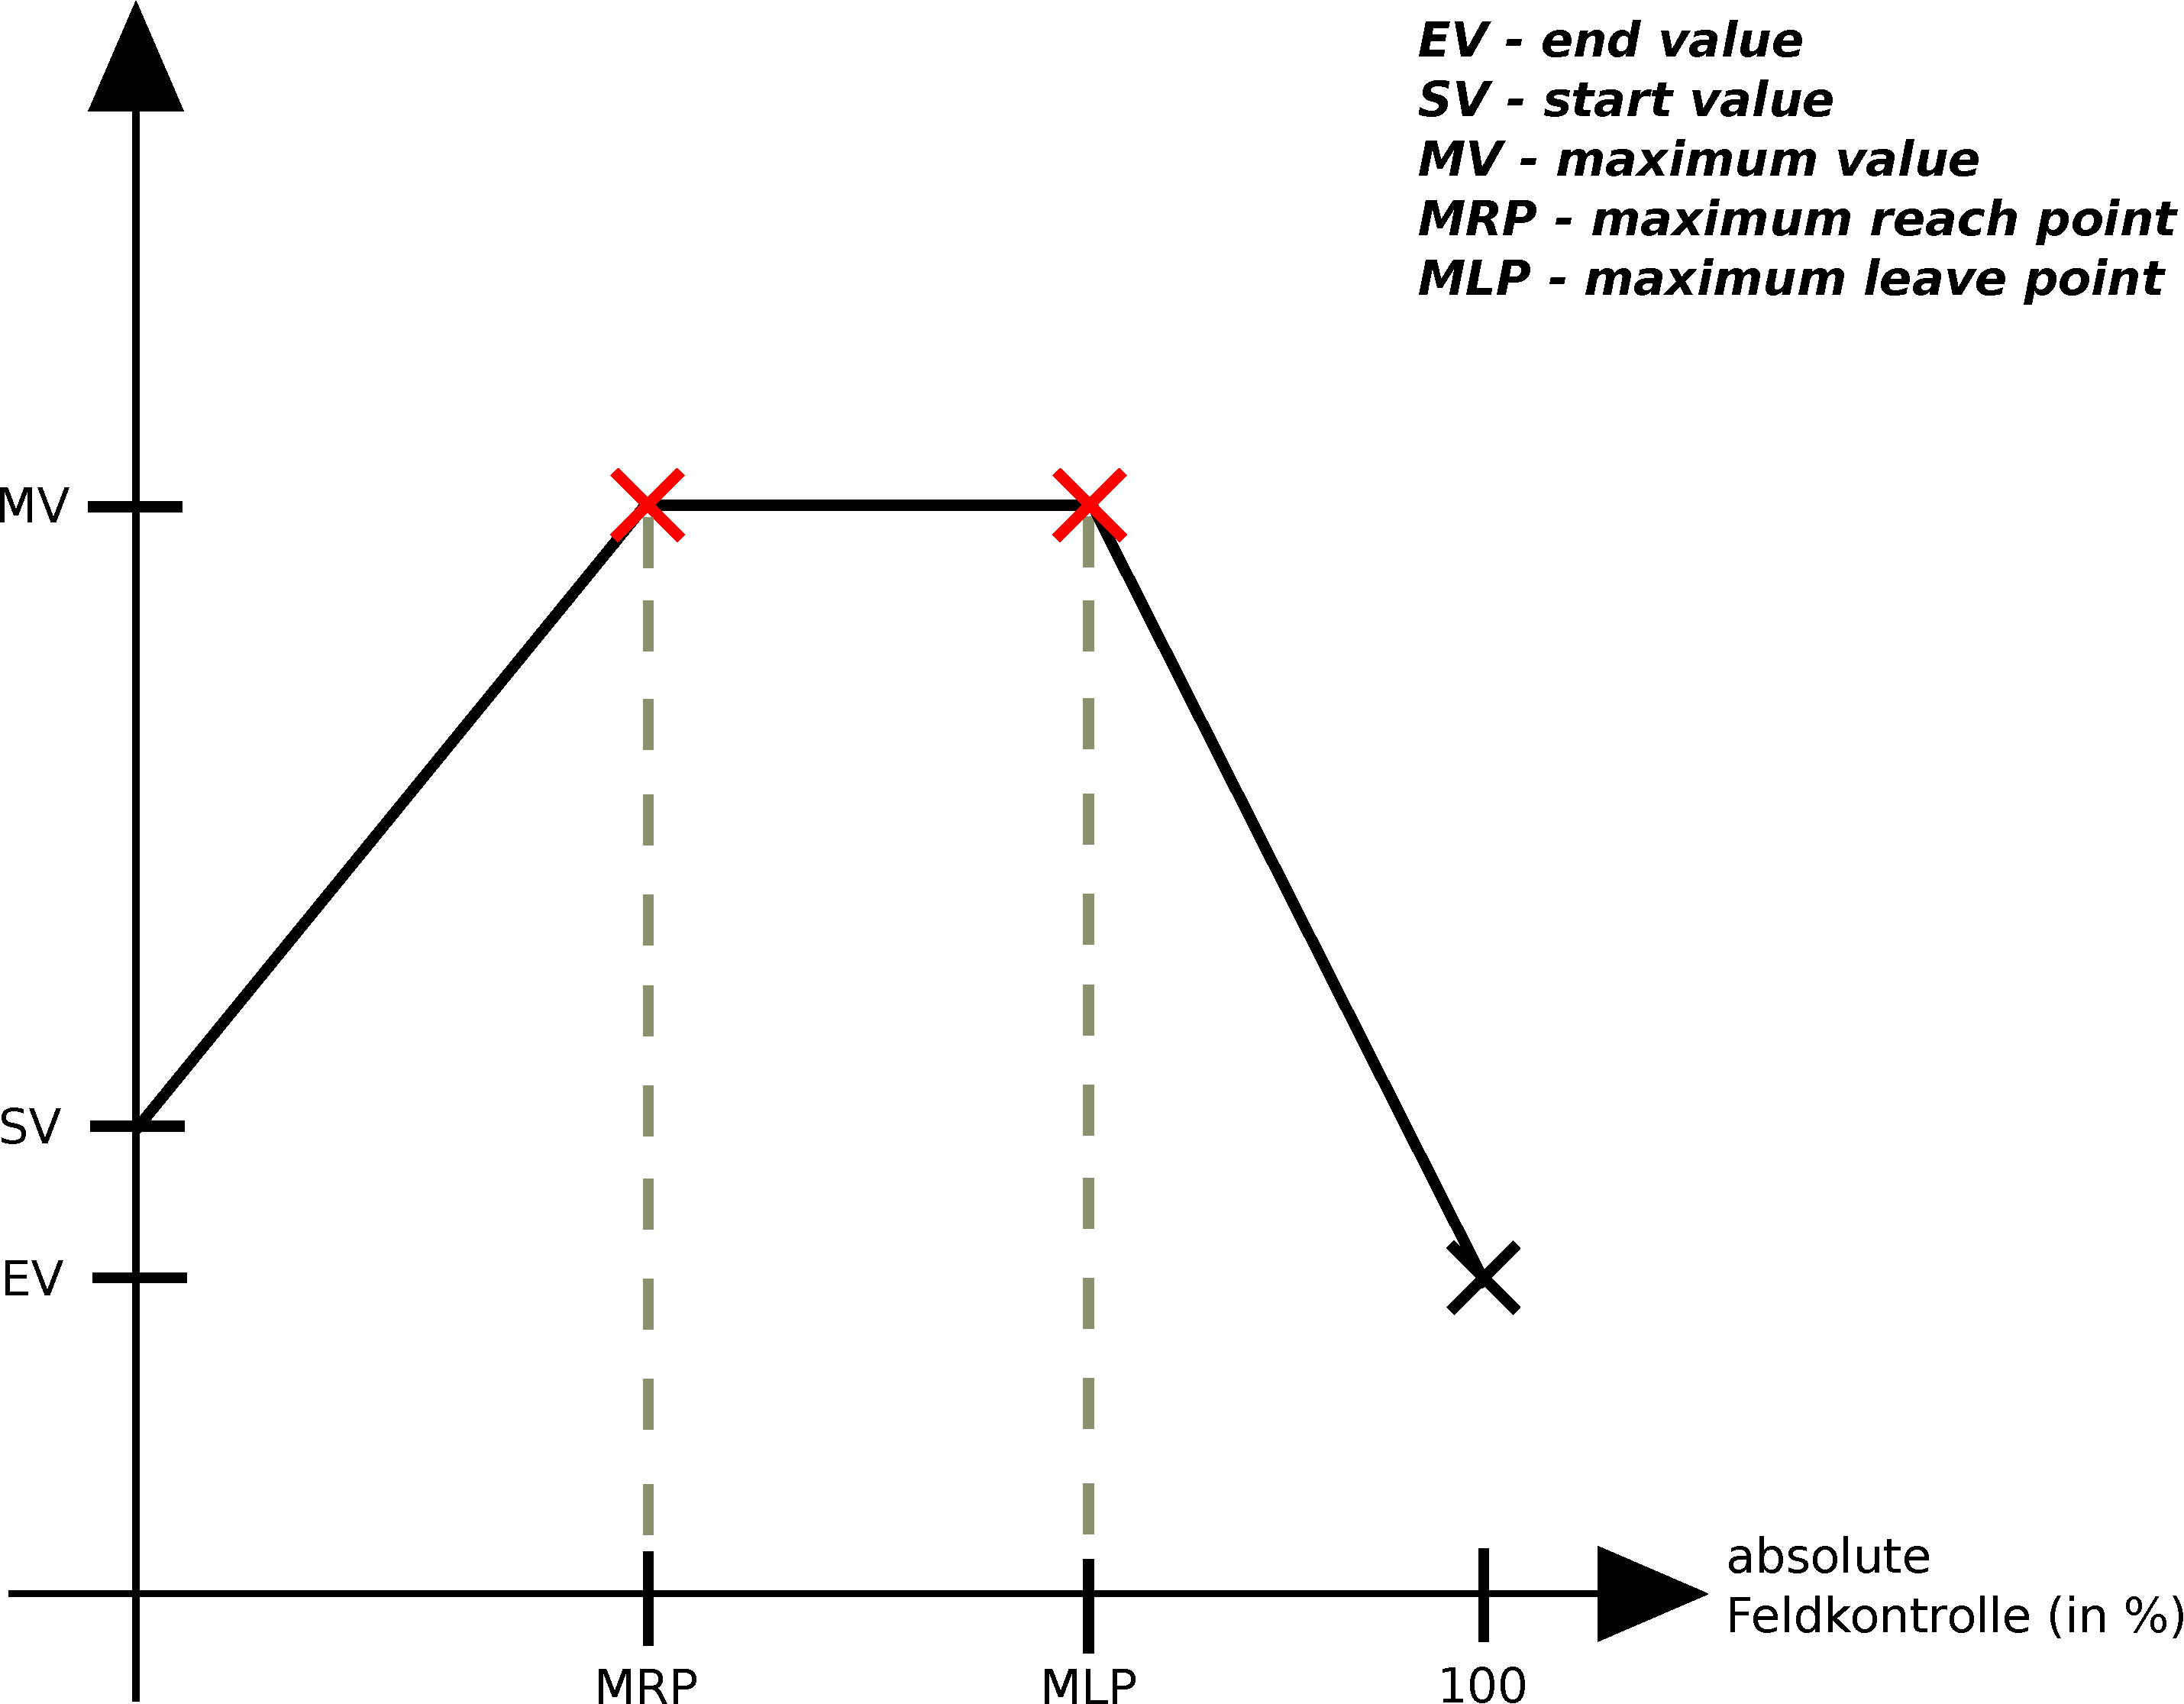
\includegraphics[width = 0.7\textwidth]{ExpectedValueGraphEdited.pdf}
\end{frame}

%--------------------------------------------------

\begin{frame}
\frametitle{Bsp. Wichtigkeitsfunktion - Anzahl eigener Steine}
\centering
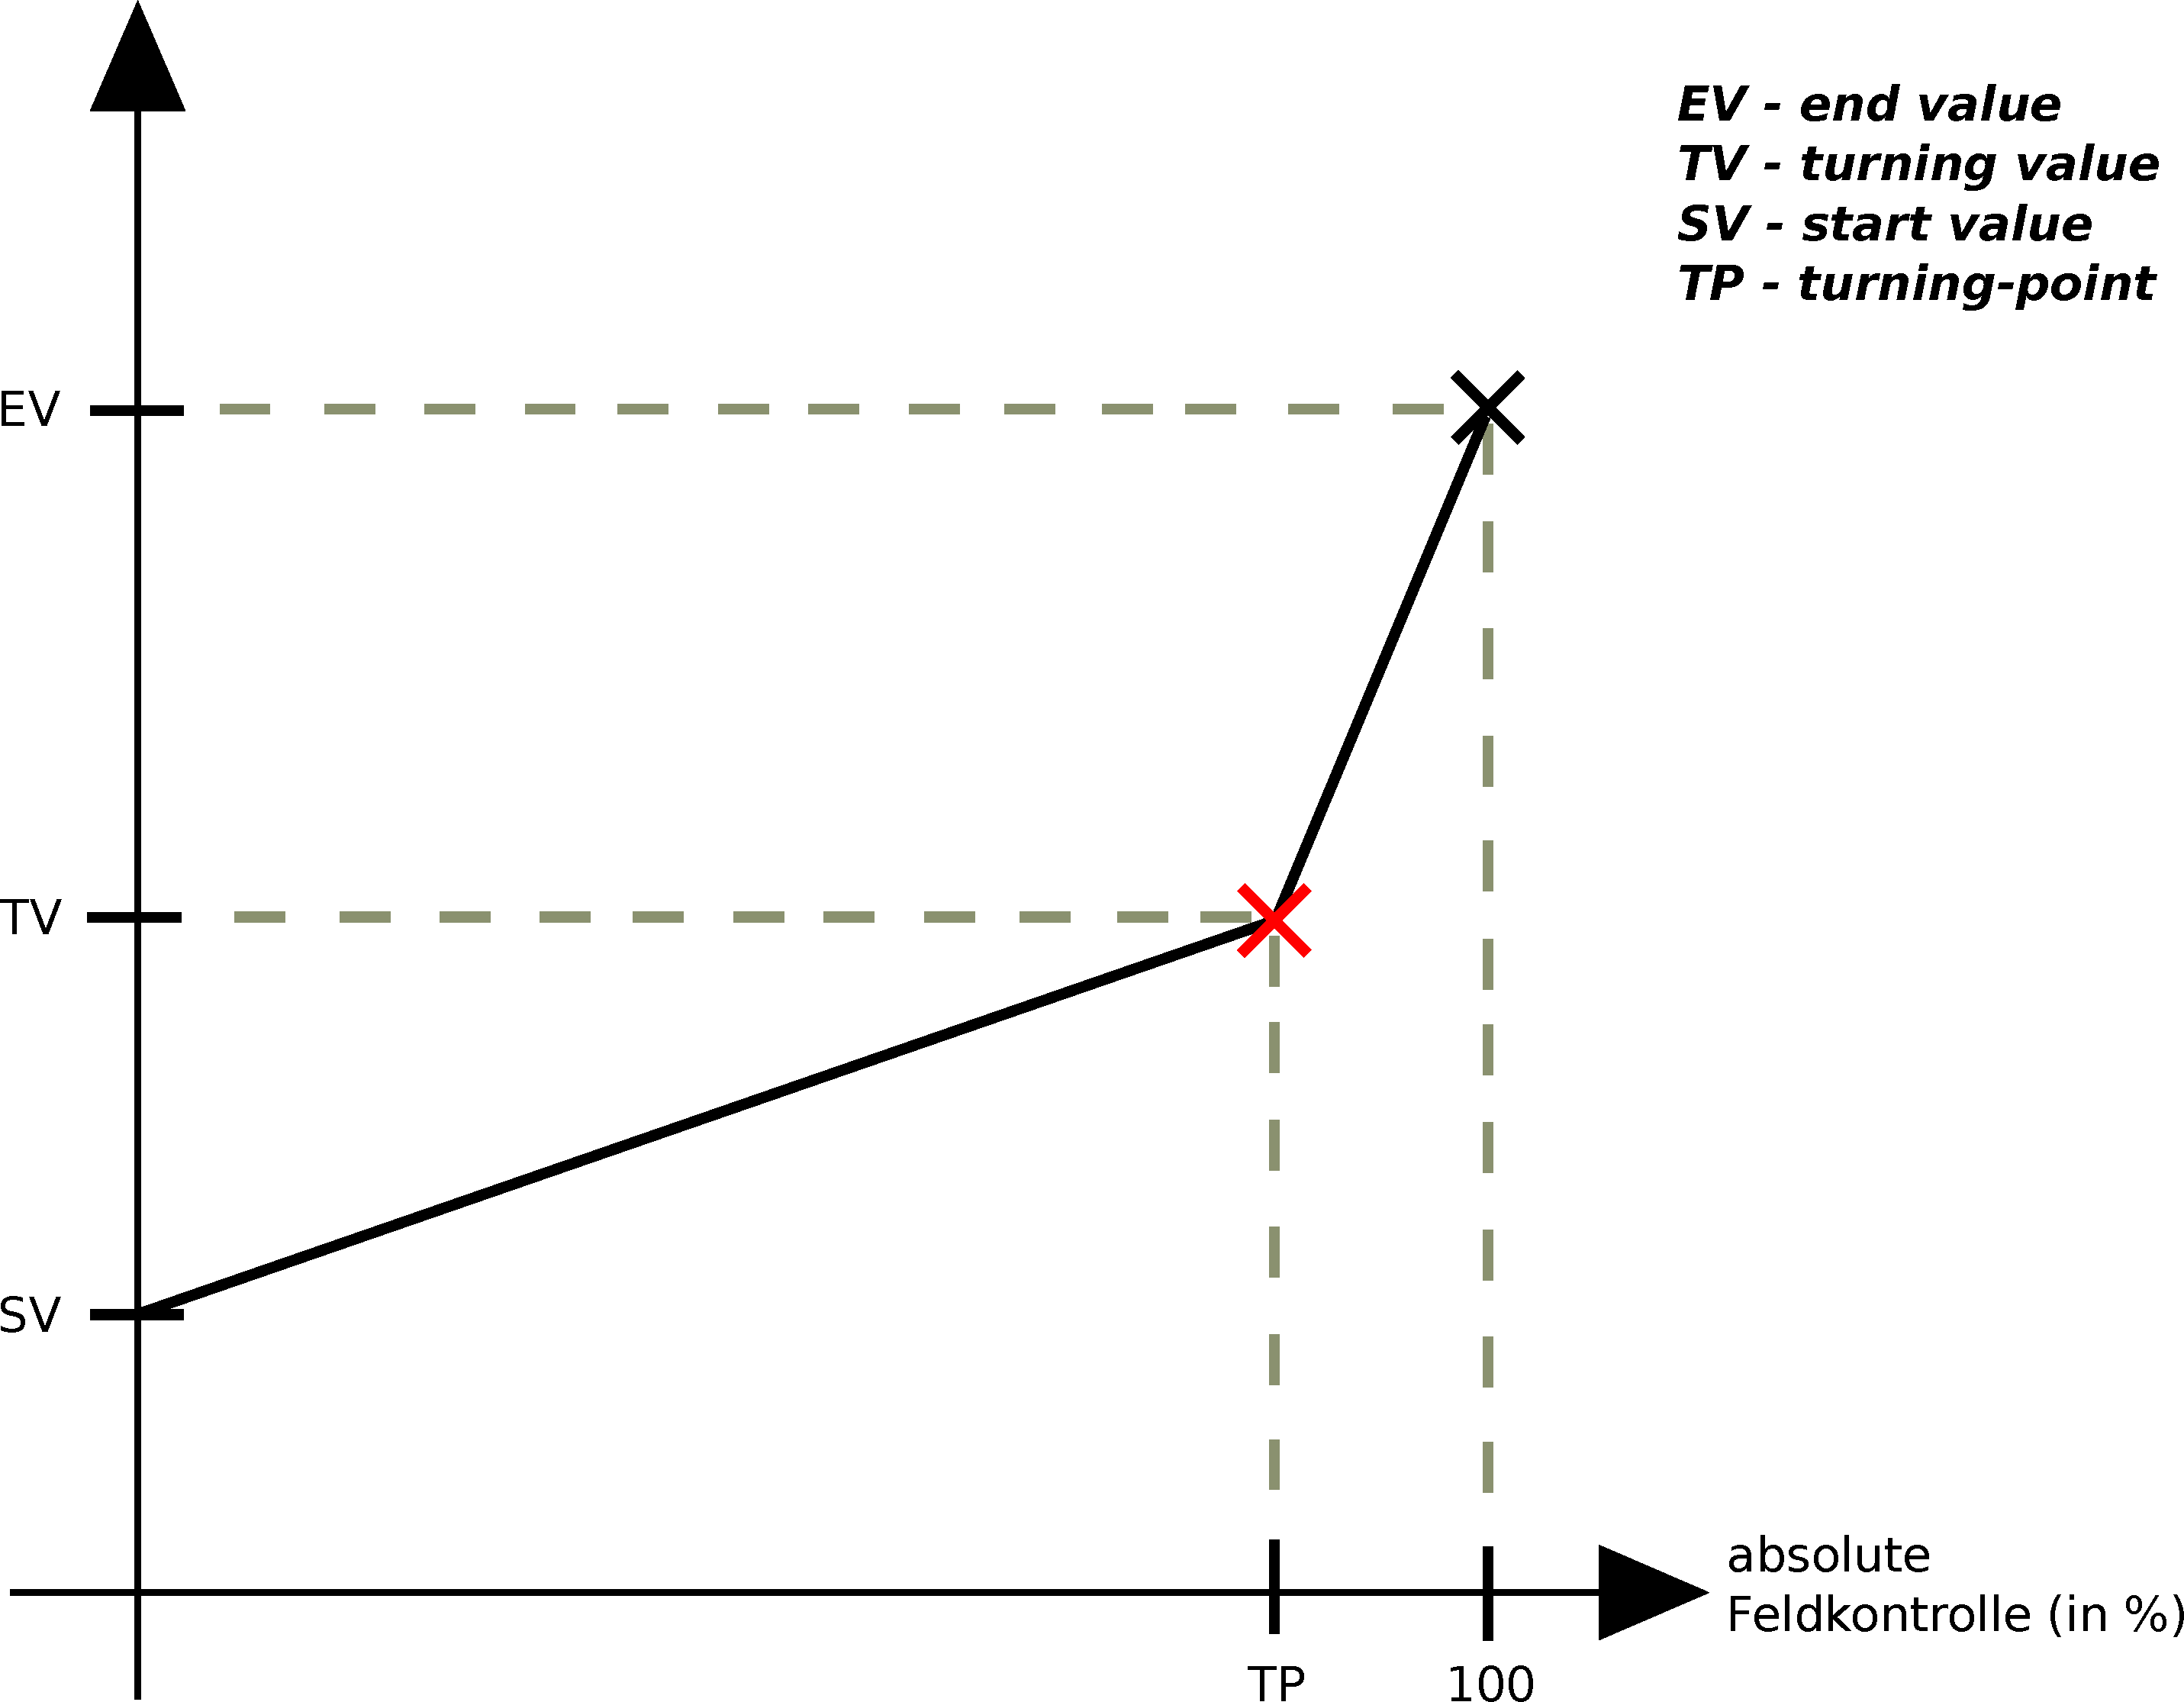
\includegraphics[width = 0.7\textwidth]{ImportanceFunctionGraph.pdf}
\end{frame}

%--------------------------------------------------
%--------------------------------------------------
%--------------------------------------------------




\end{document} 